\documentclass[tikz]{standalone}

\usetikzlibrary{arrows.meta,positioning}

\begin{document}
	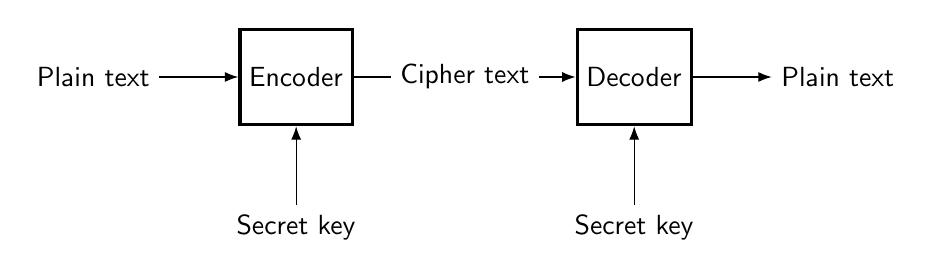
\begin{tikzpicture}[
		arrow/.style={-Latex},
		block/.style={draw, very thick, fill=white, minimum height=8ex, minimum width=3.5em},
	]
		\coordinate (in) at (0,0);
		\node (pla) [right=of in] {\textsf{Plain text}};
		\node (enc) [block, right=of pla] {\textsf{Encoder}};
		\node (dec) [block, right=8em of enc] {\textsf{Decoder}};
		\node (plb) [right=of dec] {\textsf{Plain text}};
		\coordinate[right=of plb] (out);
		
		\node (keya) [below=of enc] {\textsf{Secret key}};
		\node (keyb) [below=of dec] {\textsf{Secret key}};
		
		\draw[arrow] (pla) -- (enc);
		\draw[arrow] (enc) -- (dec) node[midway, fill=white] {\textsf{Cipher text}};
		\draw[arrow] (dec) -- (plb);
		\draw[arrow] (keya) -- (enc);
		\draw[arrow] (keyb) -- (dec);
	\end{tikzpicture}
\end{document}
